\documentclass[letterpaper, 12pt]{article}

\usepackage[normalem]{ulem}
\usepackage{scrextend}	% for the indented environment
\usepackage{amsmath,amsthm,amssymb,amsfonts}
\usepackage{graphicx, caption, subcaption}
\usepackage{hyperref}
\usepackage[top=1in, bottom=1in, left=1in, right=1in]{geometry}

\newcommand{\figurepath}{../../Figures}

% make everything 12pt font
\let\Huge\normalsize
\let\huge\normalsize
\let\LARGE\normalsize
\let\Large\normalsize
\let\large\normalsize
\let\small\normalsize
\let\footnotesize\normalsize
\let\scriptsize\normalsize
\let\tiny\normalsize

% Make everything single spacing
\linespread{1.0}

\begin{document}
%Header-Make sure you update this information!!!!
\noindent
\textbf{Study and Comparison of the Neuroidal Model} \hfill \newline Cathy Chen and Stefan Keselj \\
COS511 Final Project Report \\
Due May 15, 2018

\section{Introduction}
For our project we chose to study a new topic, a biologically plausible model of learning proposed by Les Valiant in 1994 \cite{valiant_circuits_1994}. Our study drew primarily from Valiant's book presenting this model (\textit{Circuits of the Mind}), as well as a few follow-up papers from Valiant and Papadimitriou \& Vempala. In this report we present a concise summary of our studies, describing the model, relevant algorithms, and methods of analysis, and we implement two algorithms on a simple model. We then compare mechanisms of this model to hypotheses about the human brain and to modern artificial neural networks.

\section{Neuroidal Model}\label{sec:model}
In this section we summarize our understanding of the neuroidal model. Our understanding primarily draws from \cite{valiant_circuits_1994, valiant_memorization_2005, papadimitriou_cortical_2015}.

The neuroidal model consists of a system of \underline{neurons} and \underline{synapses} which can be modeled as a weighted directed graph in which nodes represent neurons and edges represent synapses. Each neuron $i$ has a state $s_i$ containing three variables: a threshold $T\in\mathbb{R}_{>0}$, a categorical memory variable $q$, and an indicator variable $f$ that says whether the network is firing at that timestep. (In more complex versions of the model, $T\in\mathbb{R}^\gamma$, for $\gamma\in\mathbb{Z}$, which allows each neuron to store more information.) The synapse from neuron $i$ to neuron $j$ is represented by $w_{ji}\in W$, where $W$ may be a set such as $\mathbb{R}$ or $\{0,1\}$. In some versions of the model, each synapse also contains a memory state $qq$.

Each conceptual \underline{item} is represented by a group of $r$ neurons. The firing of an item's neurons denotes that the activation of the item (in terms of cognition, this means the system is ``thinking about" this item). 

\begin{figure}[!htb]
\centering
\begin{subfigure}[b]{0.45\textwidth}
      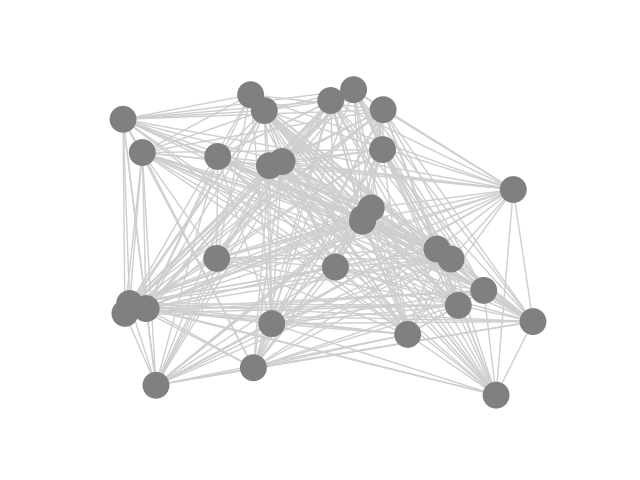
\includegraphics[width=\textwidth]{\figurepath/initialmodel.png}
      \caption*{Randomly initialized network.}
\end{subfigure}
\begin{subfigure}[b]{0.45\textwidth}
      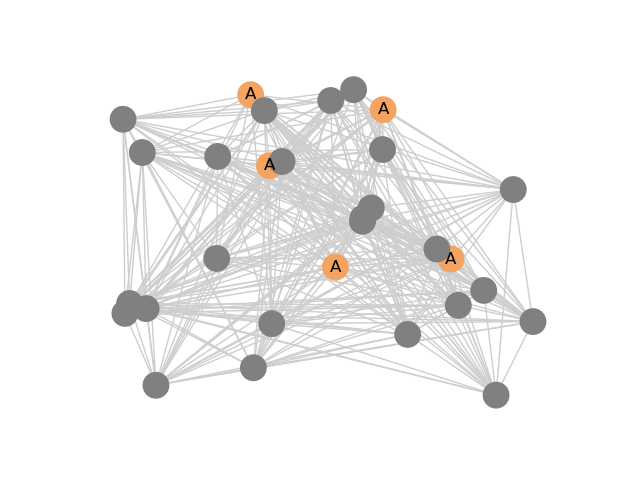
\includegraphics[width=\textwidth]{\figurepath/itemrepresentation.png}
      \caption*{$r$ neurons represent item $A$.}
\end{subfigure}
\caption{Item representation in a neuroidal network.}
\end{figure}

The system operates with discrete timesteps and all neuroid and synapse states update at each timestep according to predefined functions. This model uses \underline{vicinal} algorithms, meaning that these predefined functions are local: each neuron's update depends only on its own state, the firing of adjacent neurons, and the weights connecting the neuron and its neighbors. The functions have the form $s_{i,t+1}=\delta(s_{i,t},w_i)$, $w_{ji,t+1}=\lambda(s_i,w_i,w_{ji},f_j)$, where $w_i$ is the sum over all $w_{ki}$ for all firing neurons $k$. In particular, neuron firing spreads through synapses according to the following update rule: neuron $i$ fires if $w_i>T$. Once a neuron fires it stops firing after a pre-determined number of timesteps; in more complex models, a neuron may be blocked from firing again for a certain number of timesteps after firing.

In \cite{valiant_circuits_1994} Valiant describes four modes of learning that result from two dichotomies: one between memorization (storing explicitly provided or logically deduced information) and inductive learning (acquiring knowledge more general than the explicitly provided examples), and the other between supervised (learning from labeled examples) and unsupervised (learning from unlabeled examples) learning. Under these dichotomies, the example-based learning and PAC learning framework that we studied in COS511 fall into supervised inductive learning.

Using the neuroidal model, Valiant presents algorithms that perform all four modes of learning. He constructs algorithms that allow a neuroidal network to recognize an input after a single presentation (unsupervised memorization), associating two items (supervised memorization), learning functions of a particular class from examples (supervised inductive learning), and learning statistical correlations from item presentations (unsupervised inductive learning).

A learning system can use various \underline{peripherals} to perceive and attend to various items, store intermediate information, and organize the longer-scale timing needed in various algorithms. Valiant suggests that the combination of peripherals and of knowledge gained through memorization and inductive learning could allow for higher-level reasoning in a neuroidal model.

\section{Selected Algorithms}\label{sec:selected_algorithms}
Our study focused on the $JOIN$ and $LINK$ algorithms, which respectively implement unsupervised and supervised memorization (in terms of Valiant's dichotomies) and forming memories and associations (in terms of cognitive functions) \cite{valiant_circuits_1994, papadimitriou_cortical_2015}. In this section, we provide a high-level overview of these algorithms and our implementation of these two functions, as well as an extension of Valiant's work the proposed a new function.

We assume that networks have two modes, a ``learning" mode in which the network stores some knowledge, and an ``execution" mode in which neurons fire if their total incoming firing falls above some threshold. 

The $JOIN$ algorithm learns a conjunction of two items ``$A$" and ``$B$". During the learning mode the network's representations of $A$ and $B$ fire, and the network creates a new item ``$C$" that represents the conjunction of $A$ and $B$. Then in the execution mode the network's representation of $C$ will fire whenever the network's representations of $A$ and $B$ fire. For instance, if $A$ represents that item ``ice" and $B$ represents the item ``cream" then $JOIN(A,B)$ could form a representation of the item ``ice cream", and seeing ``ice" and ``cream" together would activate the representation of the thought ``ice cream" (rather than the separate thoughts ``ice" and ``cream").

The $LINK$ algorithm learns an association of two items ``$A$" and ``$B$". After storing $LINK(A,B)$ in the learning mode, the network will activate $B$ when $A$ is activated (in the execution mode). For instance, if $A$ represents the idea ``bell" and $B$ represents the idea ``food", then $LINK(A,B)$ would form an association of ``food" with ``bell". This algorithm involves the use of \underline{relay nodes} which act as an intermediary between $A$ and $B$, firing in response to $A$ and in turn causing $B$ to fire.

\subsection{Implementation and Simulation}
We implement algorithms that accomplish the $JOIN$ and $LINK$ functions according to specifics described in \cite{valiant_memorization_2005} and provide implementation and algorithm details on \href{https://github.com/cchen23/neuroidal_model_project/tree/master/Code}{github}.

We simulate these algorithms on neuroidal models containing $n$ neurons, $r$ neurons to represent each item we create. We initialize the network such that each pair of neurons has probability $p$ of being connected, choose a threshold $T=100$ for each neuron, and constrain the network to have maximum synaptic strength $\frac{T}{k}$. In our visualizations, a yellow outline denotes a firing neuron.

\begin{figure}[!htb]
\centering
\begin{subfigure}[b]{0.45\textwidth}
      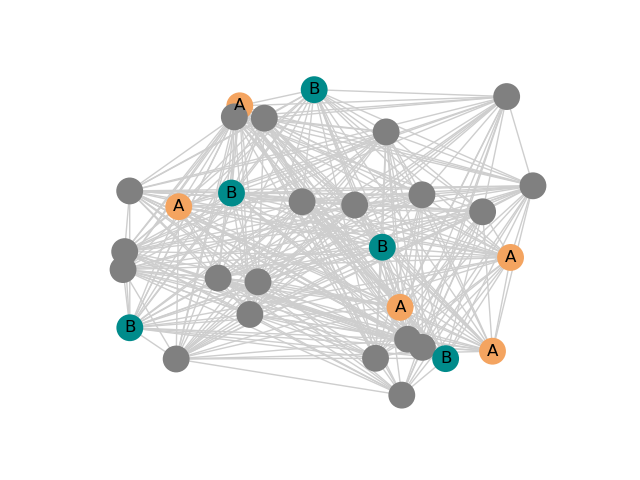
\includegraphics[width=\textwidth]{\figurepath/beforeJOIN.png}
      \caption*{Network before learning $JOIN(A,B)$}
\end{subfigure}
\begin{subfigure}[b]{0.45\textwidth}
      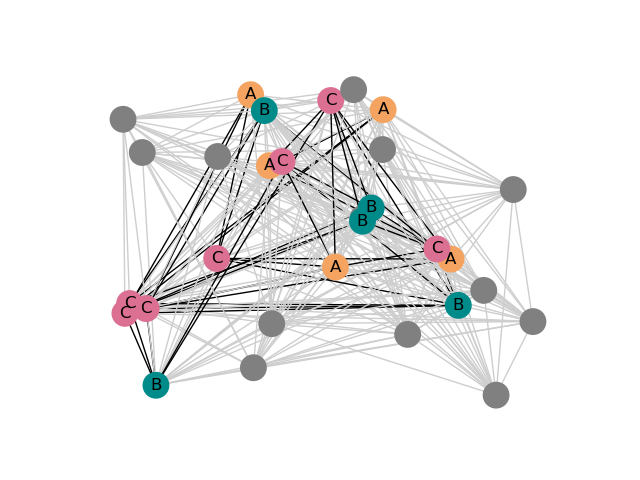
\includegraphics[width=\textwidth]{\figurepath/afterJOIN.png}
      \caption*{Network after learning $JOIN(A,B)$}
\end{subfigure}
\caption{Learning $JOIN(A,B)$ on network with $n=30,p=\frac{1}{2},k=3,r=5$. The network updates synapses from $A$ and $B$ to a set of neurons, $C$, representing $JOIN(A,B)$.}
\end{figure}

\begin{figure}[!htb]
\centering
\begin{subfigure}[b]{0.45\textwidth}
      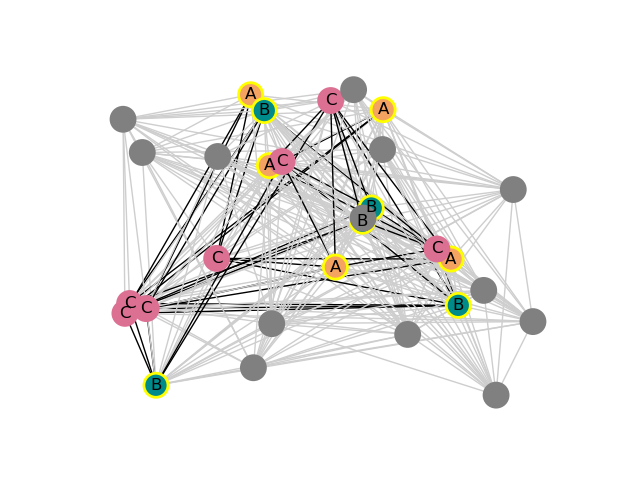
\includegraphics[width=\textwidth]{\figurepath/afterJOIN_fireAB.png}
      \caption*{$t=0$: $A$ and $B$ fire.}
\end{subfigure}
\begin{subfigure}[b]{0.45\textwidth}
      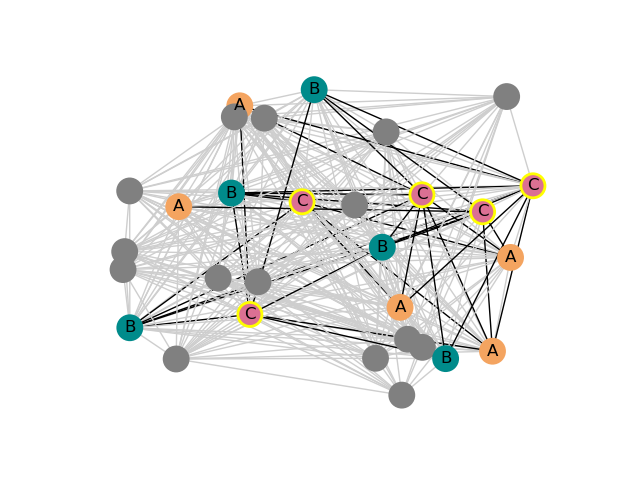
\includegraphics[width=\textwidth]{\figurepath/afterJOIN_fireAB_stepone.png}
      \caption*{$t=1$: $C$ fires.}
\end{subfigure}
\begin{subfigure}[b]{0.45\textwidth}
      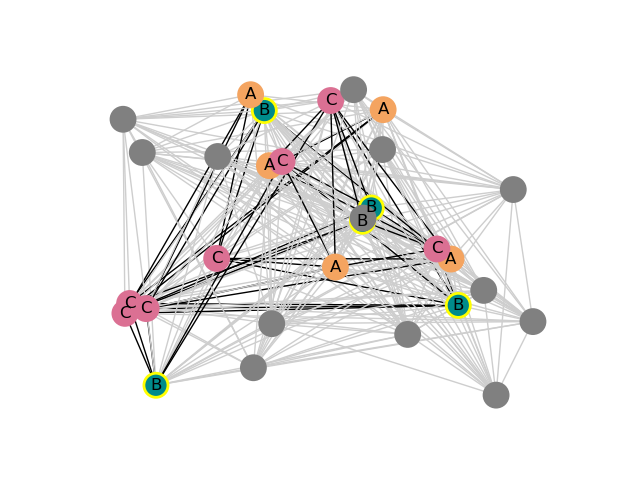
\includegraphics[width=\textwidth]{\figurepath/afterJOIN_fireB.png}
      \caption*{$t=0$: Only $B$ fires.}
\end{subfigure}
\begin{subfigure}[b]{0.45\textwidth}
      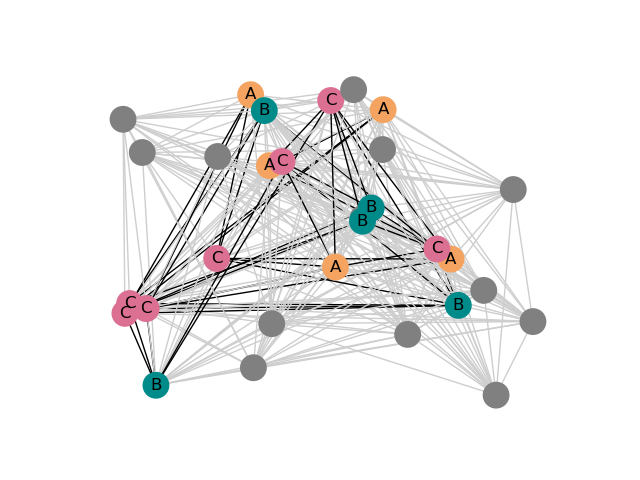
\includegraphics[width=\textwidth]{\figurepath/afterJOIN_fireB_stepone.png}
      \caption*{$t=1$: $C$ does not fire.}
\end{subfigure}
\caption{Executing $JOIN(A,B)$ on network with $n=30,p=\frac{1}{2},k=3,r=5$. $C$ represents the idea $JOIN(A,B)$: it fires if $A$ and $B$ both fire (top panels), but not if only one of $A$ and $B$ fire (bottom panels).}
\end{figure}

\begin{figure}[!htb]
\centering
\begin{subfigure}[b]{0.45\textwidth}
      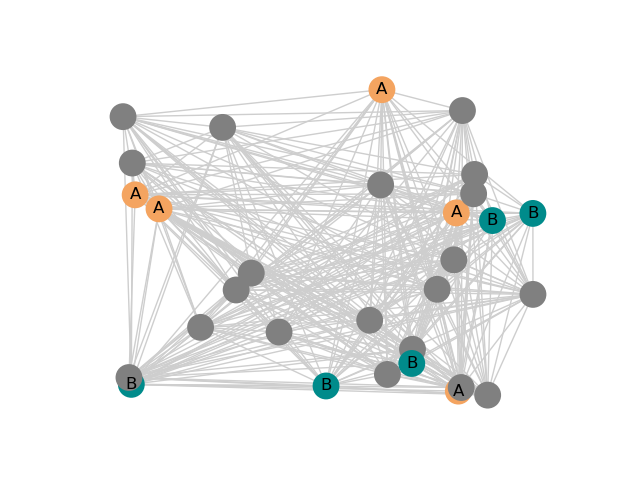
\includegraphics[width=\textwidth]{\figurepath/beforeLINK.png}
      \caption*{Network before learning $LINK(A,B)$}
\end{subfigure}
\begin{subfigure}[b]{0.45\textwidth}
      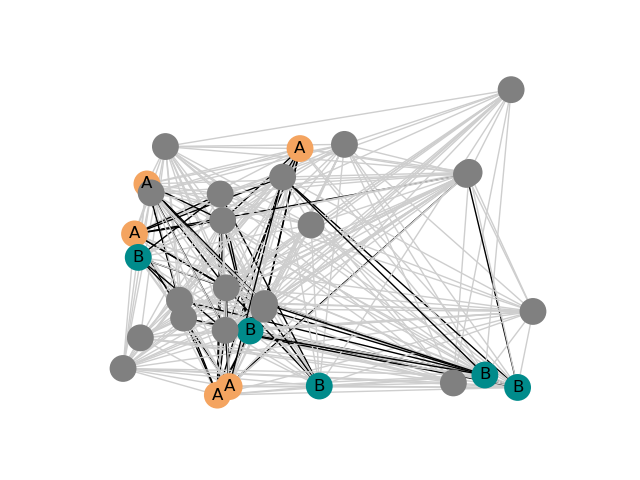
\includegraphics[width=\textwidth]{\figurepath/afterLINK.png}
      \caption*{Network after learning $LINK(A,B)$}
\end{subfigure}
\caption{Learning $LINK(A,B)$ on network with $n=30,p=\frac{1}{3},k=2,r=5$. The network updates synapses from $A$ to a set of relay neurons, and from the relay neurons to $B$.}
\end{figure}

\begin{figure}[!htb]
\centering
\begin{subfigure}[b]{0.3\textwidth}
      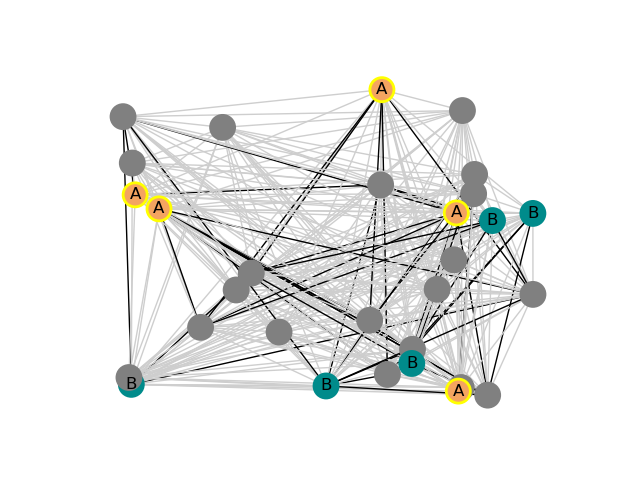
\includegraphics[width=\textwidth]{\figurepath/afterLINK_fireA.png}
      \caption*{$t=0$: $A$ fires.}
\end{subfigure}
\begin{subfigure}[b]{0.3\textwidth}
      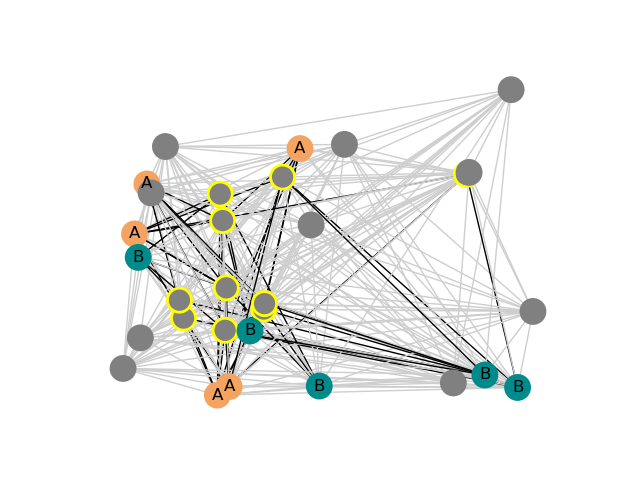
\includegraphics[width=\textwidth]{\figurepath/afterLINK_stepone.png}
      \caption*{$t=1$: Relay neurons fire.}
\end{subfigure}
\begin{subfigure}[b]{0.3\textwidth}
      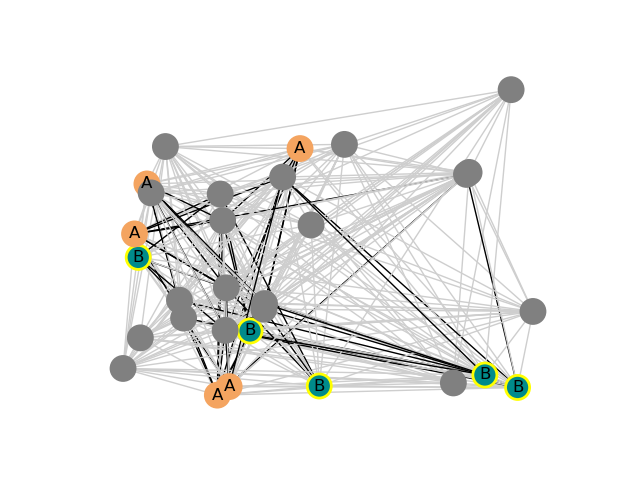
\includegraphics[width=\textwidth]{\figurepath/afterLINK_steptwo.png}
      \caption*{$t=2$: $B$ fires.}
\end{subfigure}
\caption{Executing $LINK(A,B)$ on network with $n=30,p=\frac{1}{3},k=2,r=5$. $A$ firing causes the relay neurons to fire, which in turn cause $B$ to fire.}
\end{figure}

\subsection{Extension by Papadimitriou and Vempala}\label{sec:pjoin}
Papadimitriou and Vempala \cite{papadimitriou_cortical_2015} extend Valiant's $JOIN$ and $LINK$ operations, adding an additional $PJOIN$ operation. Beyond associating or memorizing pairs of items the $PJOIN$ operation can memorize $n$-length binary patterns, meaning that it creates an item that fires when the network receives the pattern. Papadimitriou and Vempala motivate this algorithm by the combinatorial $JOIN$s required to solve this memorization task using only $JOIN$ and $LINK$; this inefficiency is especially important since the human brain operates on fast timescales, rendering algorithms requiring more than a small number of steps biologically infeasible. Rather than requiring $A$ and $B$ to fire for $C$ to fire (as in the case of $JOIN(A, B)$), after $C$ is created by $PJOIN(A,B)$ if $A$ fires, $C$ will enter a state such that it will fire if only $B$ fires at a later time; Papadimitriou and Vempala refer to this as \underline{mobilizing} $B$. Moreover, this mobilization continues down a chain of $PJOIN$s starting from $B$ and its $PJOIN$ed items. Using this algorithm adds a predictive element to neuroidal model algorithms, allowing efficient memorization of binary patterns.

\subsection{Algorithm Analysis}
For the algorithms to be useful, they must fulfill certain conditions. For $JOIN$, we want it to be highly probable that the representation $C$ also has $r$ items, that a large majority of the neurons representing $C$ are not active if $A$ and $B$ are not active, and that the representations of $A$ and $B$ only fire if the system is actually thinking of items $A$ and $B$. For $LINK$, we want it to be highly probable that if $A$ is not active then $B$ will not activate, that an $B$ will not fire in response to some item with which it is not linked, and that there are sufficient relay nodes to establish a link between $A$ and $B$. By assuming a network randomly initialized to connect two neurons with probability $p$ we can model connections as flips of a weighted coin, and use the PDF of a binomial distribution to compute that algorithm fulfills the maximum or minimum number of connections \cite{valiant_memorization_2005}. For example we can express the desired characteristic that, in a system with synapse strength at most $\frac{1}{k}$ and item size $r$, the item created by $JOIN(A, B)$ has $r$ neurons, as that the expected number of neurons with at least $k$ synapses to both $A$ and $B$ is $r$. In terms of coin flips, this is equivalent to there is an $\frac{r}{n}$ probability that two independent sequences of coin flips with probability $p$ of getting heads both have at least $k$ heads. Using this type of analysis, we can compute the probability that various parameters of the neuroidal network (number of neurons in the network, number of neurons per item, probability of connection, and strength of synapses) fulfill the desired parameters.

\section{Comparison to Human Brains}
Valiant's original model respects constraints posed by the human brain, such as the sparsity of connections and speed of processing in the human brain, and his comparison to experimental data from a biological system validates the biological plausibility of the neuroidal model \cite{valiant_quantitative_2006}. In this section we compare in more detail the neuroidal model and current hypotheses about learning in the human brain, particularly with respect to memory.

Like neurons in the neuroidal model, a neuron in the brain fires (where firing means that the neuron's membrane potential spikes) if the incoming signals (from other neurons, which are connected to this neuron by synapses) fall above a certain threshold value. Furthermore, researchers believe that changing synaptic weights in biological systems also serve as a mechanism for learning and forming memories, and that neurons enter a \underline{refractory period} that prevents a neuron from firing too soon after a previous firing \cite{cooper_donald_2005}. Researchers believe that the brain also uses groups of neurons to represent various items of memory \cite{schacter_richard_1978}.

Current understanding of biological learning also shows similarities to learning algorithms in the neuroidal model. For instance, in our descriptions of the $JOIN$ and $LINK$ algorithms the neuroidal system functions in two modes: one in which it acquires new knowledge, and one in which it recalls previously stored knowledge. Research about the hippocampus, an area of the brain implicated in memory, suggests that the hippocampus also uses two separate modes of operation, one for learning and one for recall \cite{treves_computational_1992}. Current work suggests that in certain areas of the brain the activation of some neurons that represent an item causes the rest of the item's neurons to activate as well in a phenomenon known as \underline{pattern completion}, and Papadimitriou and Vempala's $PJOIN$ algorithm, in which the firing of part of a $PJOIN$ed item mobilizes the complementary item and its associations, evokes this idea of prediction. Furthermore, the $PJOIN$ operation includes our previously mentioned refractory period in its algorithm to prevent predictions from traveling back to the item that originated a prediction.

In addition to similarities in neuroidal model components and algorithms, some implications of this model fit with experimental findings in the human brain. Model parameters (number of neurons in the network, number of neurons per item, probability of connection, and strength of synapses) that allow a neuroidal network to fulfill the bounds we describe in section \ref{sec:selected_algorithms} fit with current knowledge about these parameters in the brain \cite{valiant_memorization_2005, valiant_quantitative_2006}. Neuroscience research has found neurons that respond preferentially to specific stimuli (popularly known as ``grandmother neurons" or ``Jennifer Anniston neurons"), and the neuroidal model explains this phenomenon: the idea that some $r$ neurons in a network of $n$ neurons represent an item implies that there should be some probability $\frac{r}{n}$ of finding a neuron that responds to stimuli that induce a certain thought, if we randomly select neurons \cite{quiroga_invariant_2005, valiant_quantitative_2006}.

\section{Comparison to Neural Networks}
The neuroidal model shares many similarities with artificial neural networks that are currently very popular, yet there has been much less recent literature about this model than the amount about neural networks. In this section we compare the two models along two dimensions: structure and algorithms. To avoid confusion, we refer to Valiant's neuroidal model as ``neuroidal networks" and the neural networks such as those described in \cite{nielsen_neural_2015} as ``artificial neural networks". 

{\it Structure.}  The most salient similarity of Valiant's neuroidal model and artificial neural networks appear in the underlying structure. In both models, we can represent the networks as a graph with nodes as neurons and edges as synapses. In artificial neural networks, synapses consist only of the strength of connection between two neurons and neurons consist of some function of a linear combination of the inputs. The neuroidal model differs slightly, allowing memory states for each synapse and neuron (and in the version we consider, each neuron computes a simple threshold function of its inputs).

Furthermore, these two types of networks differ slightly in the arrangement of neurons. In artificial neural networks, the graph is often represented as a DAG, with neurons are organized into layers and each layer's neurons sending their signals toward later layers. In contrast, the version of the neuroidal model is less constrained, since we consider the network as a random graph with some shared probability of connection between any pair of neurons. Our study of the neuroidal model does not involve any constraints on neuron layout or connection restrictions.

{\it Algorithms.} A primary difference between algorithms in the neuroidal model and in artificial neural networks lies in the method of learning these algorithms. In artificial neural networks, specific algorithms are neither explicitly defined nor explicitly understood. We give the network some examples of inputs and correct outputs, and allow the network to learn some algorithm to reconstruct these input-output relationships using gradient descent. The only compass dictating how each parameter changes is its gradient with respect to some loss function of the overall network output; the specific sequence of synaptic updates is not explicitly defined by the person using the network. In contrast, to implement an algorithm in the neuroidal model one needs to define rules for how its neurons will behave and learn. Humans explicitly define algorithms to create operations such as $JOIN$ and $LINK$ to implement learning, algorithms in which each step makes sense on an intuitive level. This provides explicit interpretability of the neuroidal model's dynamics, since we can trace the sequence of steps it takes to acquire new knowledge, thought it means that the neuroidal model requires more specific, built-in functionality to perform learning.

\section{Conclusion}
Rather than perform neurobiological studies or behavioral experiments, Valiant proposes a computational approach of building a system that performs the desired behavior using components inspired by biology \cite{valiant_circuits_1994}. With this approach, the neuroidal model differs from work with the brain and artificial neural networks.

Unlike studies of the brain that start from specific analyses of biological components, this approach uses computational constraints to limit the space of algorithms, and finds algorithms within this space that accomplishes desired functions.

Unlike artificial neural networks which learn algorithms that are generally hard to interpret, the neuroidal model requires designing ``explicit computational mechanisms" for ``explicitly defined and possibly multiple cognitive tasks"; the need for designing \textit{explicit} mechanisms and tasks makes the neuroidal model perhaps less useful (at least at its current state) for generally solving problems, a use for which artificial neural networks have received much attention in the past few years.

Though this provides a disadvantage in terms of engineering solutions to large-scale problems, the explicit nature of the neuroidal model serves as an advantage for forming scientific hypotheses about learning. The explicit structure of the model and algorithms make the neuroidal model amenable to analyses of system parameters and capacity bounds that we mention in Section \ref{sec:model}, and the explicit nature of algorithms that we describe and implement in Section \ref{sec:selected_algorithms} allows us to more directly map the capabilities of the neuroidal model to hypotheses about how learning occurs in the human brain.

\bibliographystyle{IEEEtranS}
\bibliography{COS511}

\end{document}
